\documentclass{article}
\usepackage[utf8]{inputenc}
\usepackage{kotex}
\usepackage{adjustbox}
\usepackage{amsmath}
\usepackage{graphicx}
\usepackage{hyperref}

\title{Comparative Study of Various Tokenizers for Korean Text Processing}
\author{Sungyeon Kim}
\date{July 25, 2024}

\begin{document}

\maketitle
\begin{abstract}
In the realm of Natural Language Processing (NLP), tokenization plays a pivotal role in text analysis and understanding. This paper conducts a comparative study of various tokenizers for Korean text processing, including subword-based tokenizers like Google SentencePiece and several Korean morphological analyzers such as KoNLPy, Kkma, Komoran, MeCab, Soynlp, and Kiwi. The study aims to evaluate the performance of these tokenizers based on vocabulary size, execution speed, and accuracy, using the Naver movie review dataset for sentiment analysis. Results indicate that while subword tokenizers are efficient in handling vocabulary size and processing speed, morphological analyzers demonstrate higher accuracy due to their ability to reflect the intricate structure of the Korean language. This research highlights the importance of selecting appropriate tokenization methods to enhance the performance of NLP applications in Korean text processing and suggests future directions for combining morphological analysis with subword tokenization to achieve better results.
\end{abstract}


\section{Introduction}

\subsection{Background and Necessity of the Study}

In the field of Natural Language Processing (NLP), tokenizers play a crucial role in analyzing and understanding text. Tokenizers are responsible for dividing text into meaningful units that computers can process. In languages like Korean, where morphological analysis is important, accurate tokenization can enhance the performance of various NLP applications.

Tokenizing Korean is challenging due to its agglutinative nature, where particles and endings are attached to words. As a result, tokenization based on spaces alone may fail to properly tokenize sentences with poor spacing. Therefore, various attempts have been made to analyze Korean morphemes. This includes the tools provided in the KoNLPy package, such as kkma, Komoran, Mecab, Soynlp, and Kiwi. Accurate morpheme analysis can extract stems and enable effective tokenization.

Currently, large models primarily use subword-based tokenization like Google SentencePiece. However, better results may be obtained by first performing morphological analysis and then applying tokenization. Subword-based tokenizers, such as SentencePiece, are often complemented by morphological analyzers, as demonstrated by ETRI's KorBERT model. This suggests that combining morphological analysis with tokenization can improve Korean model performance.

Vocabulary size is a crucial factor in tokenization. Morphological analysis reduces the vocabulary size significantly compared to space-based word dictionaries, leading to reduced computational costs and faster training. Moreover, it decreases the number of parameters the model needs to tune, improving training efficiency.

\subsection{Purpose and Goal of the Study}

The purpose of this study is to compare the performance and characteristics of various tokenizers, including Google SentencePiece and Korean morphological analyzers (KoNLPy, Kkma, Komoran, MeCab, etc.). By identifying the strengths and weaknesses of each tokenizer, we aim to suggest the most suitable tokenizer for Korean text processing. While previous studies have examined various tokenizers, they have often overlooked Soynlp and Kiwi. Our goal is to compare their performance and propose usage strategies and future directions.

\subsection{Structure of the Paper}

This paper is structured as follows: Chapter 2 explains the theoretical background of tokenizers, and Chapter 3 reviews related studies. Chapter 4 introduces the experimental design and methodology, and Chapter 5 analyzes the experimental results. Finally, Chapter 6 presents conclusions and future research directions.

\section{Theoretical Background}

\subsection{Definition and Types of Tokenizers}

Tokenizers are tools that divide text into units. These units can be words, subwords, or characters, aiming to transform the text into a format that computers can process while preserving its meaning.


\subsection{Principles of Korean Tokenization}

Korean tokenization can be broadly categorized into two main approaches: subword tokenization and morphological analysis. Each approach has distinct principles and use cases, catering to different needs in natural language processing (NLP).

\subsubsection{Subword Tokenization}

Subword tokenization involves breaking down text into smaller units than words, often into subword units or character sequences. This method is particularly effective for handling out-of-vocabulary words and reducing the size of the vocabulary needed for language models.

\begin{itemize}
\item \textbf{Byte-Pair Encoding (BPE)}:
    \begin{itemize}
        \item BPE starts with individual characters and iteratively merges the most frequent pairs of symbols (characters or sequences of characters).
        \item The merging process continues until a predefined vocabulary size is reached.
        \item This approach helps to capture common subword patterns, making it effective for agglutinative languages like Korean, where many word forms can be derived from a single root.
    \end{itemize}

\item \textbf{Unigram Language Model}:
    \begin{itemize}
        \item This method models the probability of each subword unit, typically starting with a large set of candidate subwords.
        \item It iteratively removes the least probable subwords while recalculating probabilities until the desired vocabulary size is achieved.
        \item Unigram models can be more flexible than BPE as they do not rely on merging pairs but instead on optimizing subword probabilities.
   \end{itemize}

\item \textbf{Applications and Advantages}:
    \begin{itemize}
        \item Subword tokenization is particularly useful in machine translation, language modeling, and other tasks where handling a large and dynamic vocabulary is essential.
        \item It can effectively manage rare and compound words by breaking them into known subword units, ensuring that the model encounters fewer unknown tokens.
    \end{itemize}
\end{itemize}

\subsubsection{Morphological Analysis}

Morphological analysis involves segmenting and tagging the text based on its grammatical structure. This approach identifies the root forms of words and their affixes, providing a detailed understanding of the linguistic components of each token.

\begin{itemize}
\item \textbf{Morphological Segmentation}:
    \begin{itemize}
        \item The text is segmented into morphemes, which are the smallest units of meaning, including roots, prefixes, suffixes, and particles.
        \item This process requires linguistic knowledge and often utilizes pre-built dictionaries and rules specific to the language.
    \end{itemize}
\item \textbf{Part-of-Speech (POS) Tagging}:
    \begin{itemize}
        \item Each morpheme is assigned a part-of-speech tag, indicating its grammatical role (e.g., noun, verb, adjective).
        \item POS tagging helps in understanding the syntactic and semantic functions of words within sentences.
   \end{itemize}
\item \textbf{Morphological Parsing}:
    \begin{itemize}
        \item The parser analyzes the structure of words to determine their base forms and affixes.
        \item This involves identifying morphological patterns and rules, such as conjugation and inflection in verbs or declension in nouns.
    \end{itemize}
\item \textbf{Applications and Advantages}:
    \begin{itemize}
        \item Morphological analysis is essential for tasks requiring deep linguistic understanding, such as syntactic parsing, information extraction, and linguistic research.
        \item It provides precise information about word forms and their grammatical relationships, which is crucial for understanding complex language phenomena.
    \end{itemize}
\end{itemize}

\subsubsection{Comparison and Use Cases}
\begin{itemize}
\item \textbf{Subword Tokenization}:
    \begin{itemize}
        \item \textbf{Advantages}: Handles out-of-vocabulary words effectively, reduces vocabulary size, and is efficient for training large-scale language models.
        \item \textbf{Use Cases}: Machine translation, speech recognition, and any NLP task requiring robust handling of diverse and dynamic vocabularies.
    \end{itemize}
\item \textbf{Morphological Analysis}:
    \begin{itemize}
        \item \textbf{Advantages}: Provides detailed grammatical information, improves understanding of linguistic structures, and enhances accuracy in syntactic and semantic tasks.
        \item \textbf{Use Cases}: Syntactic parsing, information extraction, morphological research, and applications requiring precise linguistic analysis.
    \end{itemize}
\end{itemize}
Both subword tokenization and morphological analysis play crucial roles in processing Korean text, each suited to different aspects of natural language understanding and generation. The choice between them depends on the specific requirements of the task and the nature of the language data being handled.



\subsection{Introduction to Major Tokenizers}

\subsubsection{Google SentencePiece}

Google SentencePiece is a subword unit-based tokenizer independent of language. This data-driven approach divides input text into subword units, reducing vocabulary size and addressing the issue of rare words.

\subsubsection{Korean Morphological Analyzers}

Korean morphological analyzers divide Korean text into morphemes. Major analyzers include KoNLPy, Kkma, Komoran, and MeCab. The study will also cover Bareun and more recently developed tokenization methods such as Kiwi and Soynlp. 

    \begin{itemize}
        \item \textbf{Kkma}: a morphological analyzer and natural language processing system written in Java, developed by the Intelligent Data Systems Laboratory at Seoul National University.
        \item \textbf{Hannanum}: a morphological analyzer and POS tagger written in Java, developed by the Semantic Web Research Center at KAIST.
        \item \textbf{KOMORAN}: a relatively new open source Korean morphological analyzer written in Java, developed by Shineware.
        \item \textbf{MeCab}: originally a Japanese morphological analyzer and POS tagger developed by the Graduate School of Informatics in Kyoto University, was modified to MeCab-ko by the Eunjeon Project to adapt to the Korean language
        \item \textbf{Okt}: An open-source Korean morphological analyzer written in Scala, developed by Will Hohyon Ryu.
    \end{itemize}


\begin{itemize}
    \item \textbf{Bareun}: 
        \begin{itemize}
            \item Developed by Baikal AI and the Korea Press Foundation.
            \item BARN, a Korean morphological analyzer, was jointly developed by Baikal AI and the Korea Press Foundation from July 2022 to January 2023 through the “Morphological Analyzer Development Project for Media Companies”.
            \item It is said to have created a segmentation and tagging model structure utilizing transformer encoders.
        \end{itemize}
        
    \item \textbf{Kiwi}: 
        \begin{itemize}
            \item An open-source Korean morphological analyzer based on a C++ core library.
            \item Starting with Kiwi 0.5, there is also a feature that extracts strings that are presumed to be words by recognizing patterns in frequently occurring strings. The idea behind this feature is based on the Word Extraction technique from https://github.com/lovit/soynlp, which uses a combination of string-based noun probabilities to extract only words that are predicted to be nouns.
            \item It can be further customized to enable accurate tokenization through user dictionary management.
        \end{itemize}
    \item \textbf{Soynlp}: 
        \begin{itemize}
            \item Statistics-based tokenizers
            \item In addition to tokenizer, it also provides word extraction, part-of-speech, and preprocessing
            \item Since morphology-based tokenizers are vulnerable to unregistered words, soynlp can be used to solve the shortcomings of morphology-based koNLPy, just as WordPiece Model is used.
            \item Using an unsupervised learning approach to determine the boundaries of words, allowing tokenization of unregistered words
        \end{itemize}
\end{itemize}

\section{Related Research}

\subsection{Review of Existing Research}

Existing research evaluates the performance of various tokenizers using metrics such as accuracy, processing speed, and memory usage. For example, using SentencePiece for training the BERT model has been reported to be efficient in terms of vocabulary size and processing speed. In contrast, morphological analyzers reflect the complex structure of Korean, demonstrating high accuracy.

\subsection{Tokenizer Comparison Studies}

Previous studies primarily used quantitative metrics (e.g., accuracy, F1-score) to evaluate tokenizer performance. Additionally, qualitative analysis was conducted to assess the quality of tokenized text.

\section{Experimental Design}

\subsection{Dataset}

This study used the Naver movie review sentiment analysis dataset, which is balanced with positive and negative reviews, making it suitable for performance comparison. The performance metrics used were accuracy and ROC AUC.

\subsection{Experimental Environment and Tools}

The experiments were conducted using Python-based NLP tools and libraries. Each tokenizer was implemented using its respective library (KoNLPy, SentencePiece, etc.) and compared under the same environment. The experiments were performed on a Mac M2 24GB, with multiple runs to calculate average performance values.

\subsection{Preprocessing Process}

\begin{itemize}
\item We figured out that the initial sounds ㅜㅜ and ㅋㅋ can carry the meaning of emotions, so we left out letters, numbers, initial sounds, and ♥♡乃ㄹ.
\item We added code to remove multiple spaces
\item We recognized that k and kk are different Multiple initial sounds such as ㅜㅜㅜ, ㅋㅋㅋ ㅋㅋㅋ, etc. were combined into two initial sounds.
\item Empty hearts and filled hearts were replaced with filled hearts, and the number of hearts was replaced with one.
\item Repeating strings were removed, leaving only one.
\end{itemize}
The detailed code of preprocessing process can be found on github


\subsection{Modeling}
The vocab size is also a result of the performance of the tokenizer. so I varied the vocab size for each tokenizer and compared the performance of sentencepiece alone, and additionally compared the performance by vocab size.(Appendix)

The model used an LSTM model with 1 LSTM layer with 128 units, and rmsprop was used as the optimizer.
20\% of the train dataset was used as the validation dataset.
I set 20 epochs, but it tended to overfit around 8 widths.

The detailed code of the model can be found on github

\subsection{Evaluation Method}

Evaluation was conducted using both quantitative metrics and qualitative analysis.

\begin{itemize}
    \item \textbf{Quantitative Metrics}: Comparison of vocabulary size, rare word ratio, accuracy, ROC AUC, and processing speed when tokenizing the same dataset.
    \item \textbf{Qualitative Analysis}: Evaluation of the quality of tokenized text and analysis of example sentences to assess the performance of each tokenizer.
\end{itemize}

\section{Results and Analysis}

\subsection{Quantitative Evaluation}
The following observations can be made from the quantitative evaluation tables:


\subsubsection{Execution speed and Test accuracy}
Execution speed and test accuracy will also be important factors in measuring performance.
We compared the execution times of as many tokenizers as we could, and used 5 iterations and averaged them to get an accurate measure of performance.
Exec Time in the table measures the time taken to tokenize 1000 sentences from the train dataset
For time reasons, we were unable to check test acc for a few tokenizers.
In particular, in the case of Kkma, we found errors for a few characters.
We did not test Kkma on the full dataset due to its long runtime and the heavy burden of error correction.


\begin{table}[h]
    \centering
    \begin{tabular}{|l|c|c|c|}
        \hline
        Tokenizer & Exec Time (Sec) & Test Acc & \# of Train \\
        \hline
        Okt (stem=False) & 1.44 & 0.8586 & 145115 \\
        Okt (norm=True) & 4.04 & - & - \\
        Okt (stem=True) & 2.27 & 0.8613 & 145269 \\
        Okt (norm=True, stem=True) & 4.04 & - & - \\
        Kkma & 12.80 & - & - \\
        Komoran & 0.28 & 0.8544 & 143232 \\
        Mecab & 0.02 & 0.8649 & 145308 \\
        Hannanum & 2.21 & 0.8199 & 139997 \\
        Kiwi & 0.66 & 0.8648 & 148381 \\
        Bareun & 12.16 & 0.8616 & 148402 \\
        Soynlp MaxScoreTokenizer & 0.05 & 0.8570 & 147655 \\
        Soynlp LTokenizer & 0.01 & 0.8357 & 145126 \\
        SentencePiece & 0.01 & 0.8601 & 145510 \\
        \hline
    \end{tabular}
    \caption{Performance Table}
\end{table}

\begin{itemize}
    \item \textbf{Execution Time}: Measured in seconds, showing how fast each tokenizer processes the data.
    
    \begin{itemize}
        \item \textbf{Mecab}: The fastest tokenizer with an execution time of 0.02 seconds.
        \item \textbf{Soynlp LTokenizer and SentencePiece}: Also very fast with execution times of 0.01 seconds.
        \item \textbf{Kkma and Bareun}: The slowest with execution times of 12.80 and 12.16 seconds, respectively.
    \end{itemize}

    \item \textbf{Test Accuracy}: Indicates the model's accuracy on the test dataset.
    \begin{itemize}
        \item \textbf{Mecab}: Achieves the highest test accuracy at 0.8649.
        \item \textbf{Kiwi}: Also performs well with a test accuracy of 0.8648.
        \item \textbf{Other tokenizers}: Show varying accuracies, with Hannanum being the lowest at 0.8199.
    \end{itemize}
    \item \textbf{Number of Training Tokens}: Represents the total number of tokens produced for training.
    \begin{itemize}
        \item \textbf{Komoran and Soynlp LTokenizer}: Produce fewer tokens, suggesting they might segment text into larger units.
        \item \textbf{Kiwi and Bareun}: Generate the highest number of tokens, indicating finer segmentation.
    \end{itemize}
\end{itemize}

    Overall, the tables highlight the trade-offs between tokenizer efficiency (execution time and vocabulary size) and effectiveness (test accuracy and rare words frequency). Tokenizers like Mecab and Kiwi appear to balance these factors well, demonstrating both high accuracy and efficiency.

\subsubsection{Tokenizer Result (Detailed)}
\begin{itemize}
    \item \textbf{Vocabulary Size Variation}: The vocabulary size varies across different tokenizers, which can be indicative of their approach to tokenization. A smaller vocabulary size generally suggests a more efficient tokenizer, capable of reducing the total number of unique tokens.

    \item \textbf{Rare Words Analysis}: The number and frequency of rare words are crucial indicators. A lower count of rare words can imply that the tokenizer effectively segments the text into meaningful units, ensuring fewer tokens are discarded due to rarity.
\end{itemize}


\begin{table}[htbp]
\centering
\begin{adjustbox}{height=150pt, max width=\textwidth}
\begin{tabular}{|l|c|c|c|c|c|}
\hline
    \textbf{Tokenizer} & \textbf{Vocab Size} & \textbf{\# of Rare Words} & \textbf{Rare Words Freq(\%)} & \textbf{Total Vocab} \\ 
\hline
     Okt (stem=True)& 19,805 & 25,753 & 1.64 & 45,557 \\ 
     Kiwi           & 17,879 & 29,065 & 1.29 & 46,943 \\
    Mecab           & 21,741 & 28,464 & 1.46 & 50,204 \\ 
    Komoran        & 18,190  & 36,854 & 1.64 & 55,043 \\
    Bareun         & 20,643  & 46,039 & 2.07 & 66,681 \\ 
    Okt (stem=False) & 32,667 & 68,875 & 4.27 & 101,541 \\
    Soynlp MaxScoreTokenizer & 28,370    & 138,873 & 9.04  & 167,242\\ 
    Hannanum           & 23,529 & 158,670   & 8.20  & 182,198     \\
    Soynlp LTokenizer   & 29,656 & 205,513  & 15.07 & 235,168     \\ 
\hline
\end{tabular}
\end{adjustbox}
\caption{Tokenizer Result}
\label{tab:vocabulary}
\end{table}

[Table 2] displays the detailed tokenization result for all train sentences(145510 sentences) using various tokenizers. Here are the summarized characteristics and performance insights for each tokenizer:

\begin{itemize}
    \item \textbf{Okt (stem=True)}: This tokenizer has a relatively small vocabulary size and a moderate number of rare words, indicating it performs well in balancing vocabulary reduction and token meaningfulness.
    
    \item \textbf{Kiwi}: Exhibits the smallest vocabulary size among the tokenizers and a low percentage of rare words, suggesting high efficiency in tokenization.
    
    \item \textbf{Mecab}: Shows a slightly larger vocabulary size than Kiwi but maintains a low frequency of rare words, indicating good performance.
    
    \item \textbf{Komoran}: Has a moderate vocabulary size and a higher number of rare words compared to Kiwi and Mecab, implying it may produce more unique tokens that are not frequently used.
    
    \item \textbf{Bareun}: Displays a larger vocabulary size and a higher frequency of rare words, suggesting it may create many unique tokens.
    
    \item \textbf{Okt (stem=False)}: This configuration has the largest vocabulary size and the highest percentage of rare words, indicating less efficient tokenization without stemming.
    
    \item \textbf{Soynlp MaxScoreTokenizer and Soynlp LTokenizer}: Both have very large vocabulary sizes and high frequencies of rare words, which may lead to inefficiencies in text processing.
\end{itemize}


\subsection{Qualitative Analysis}

\begin{figure}
        \centering
        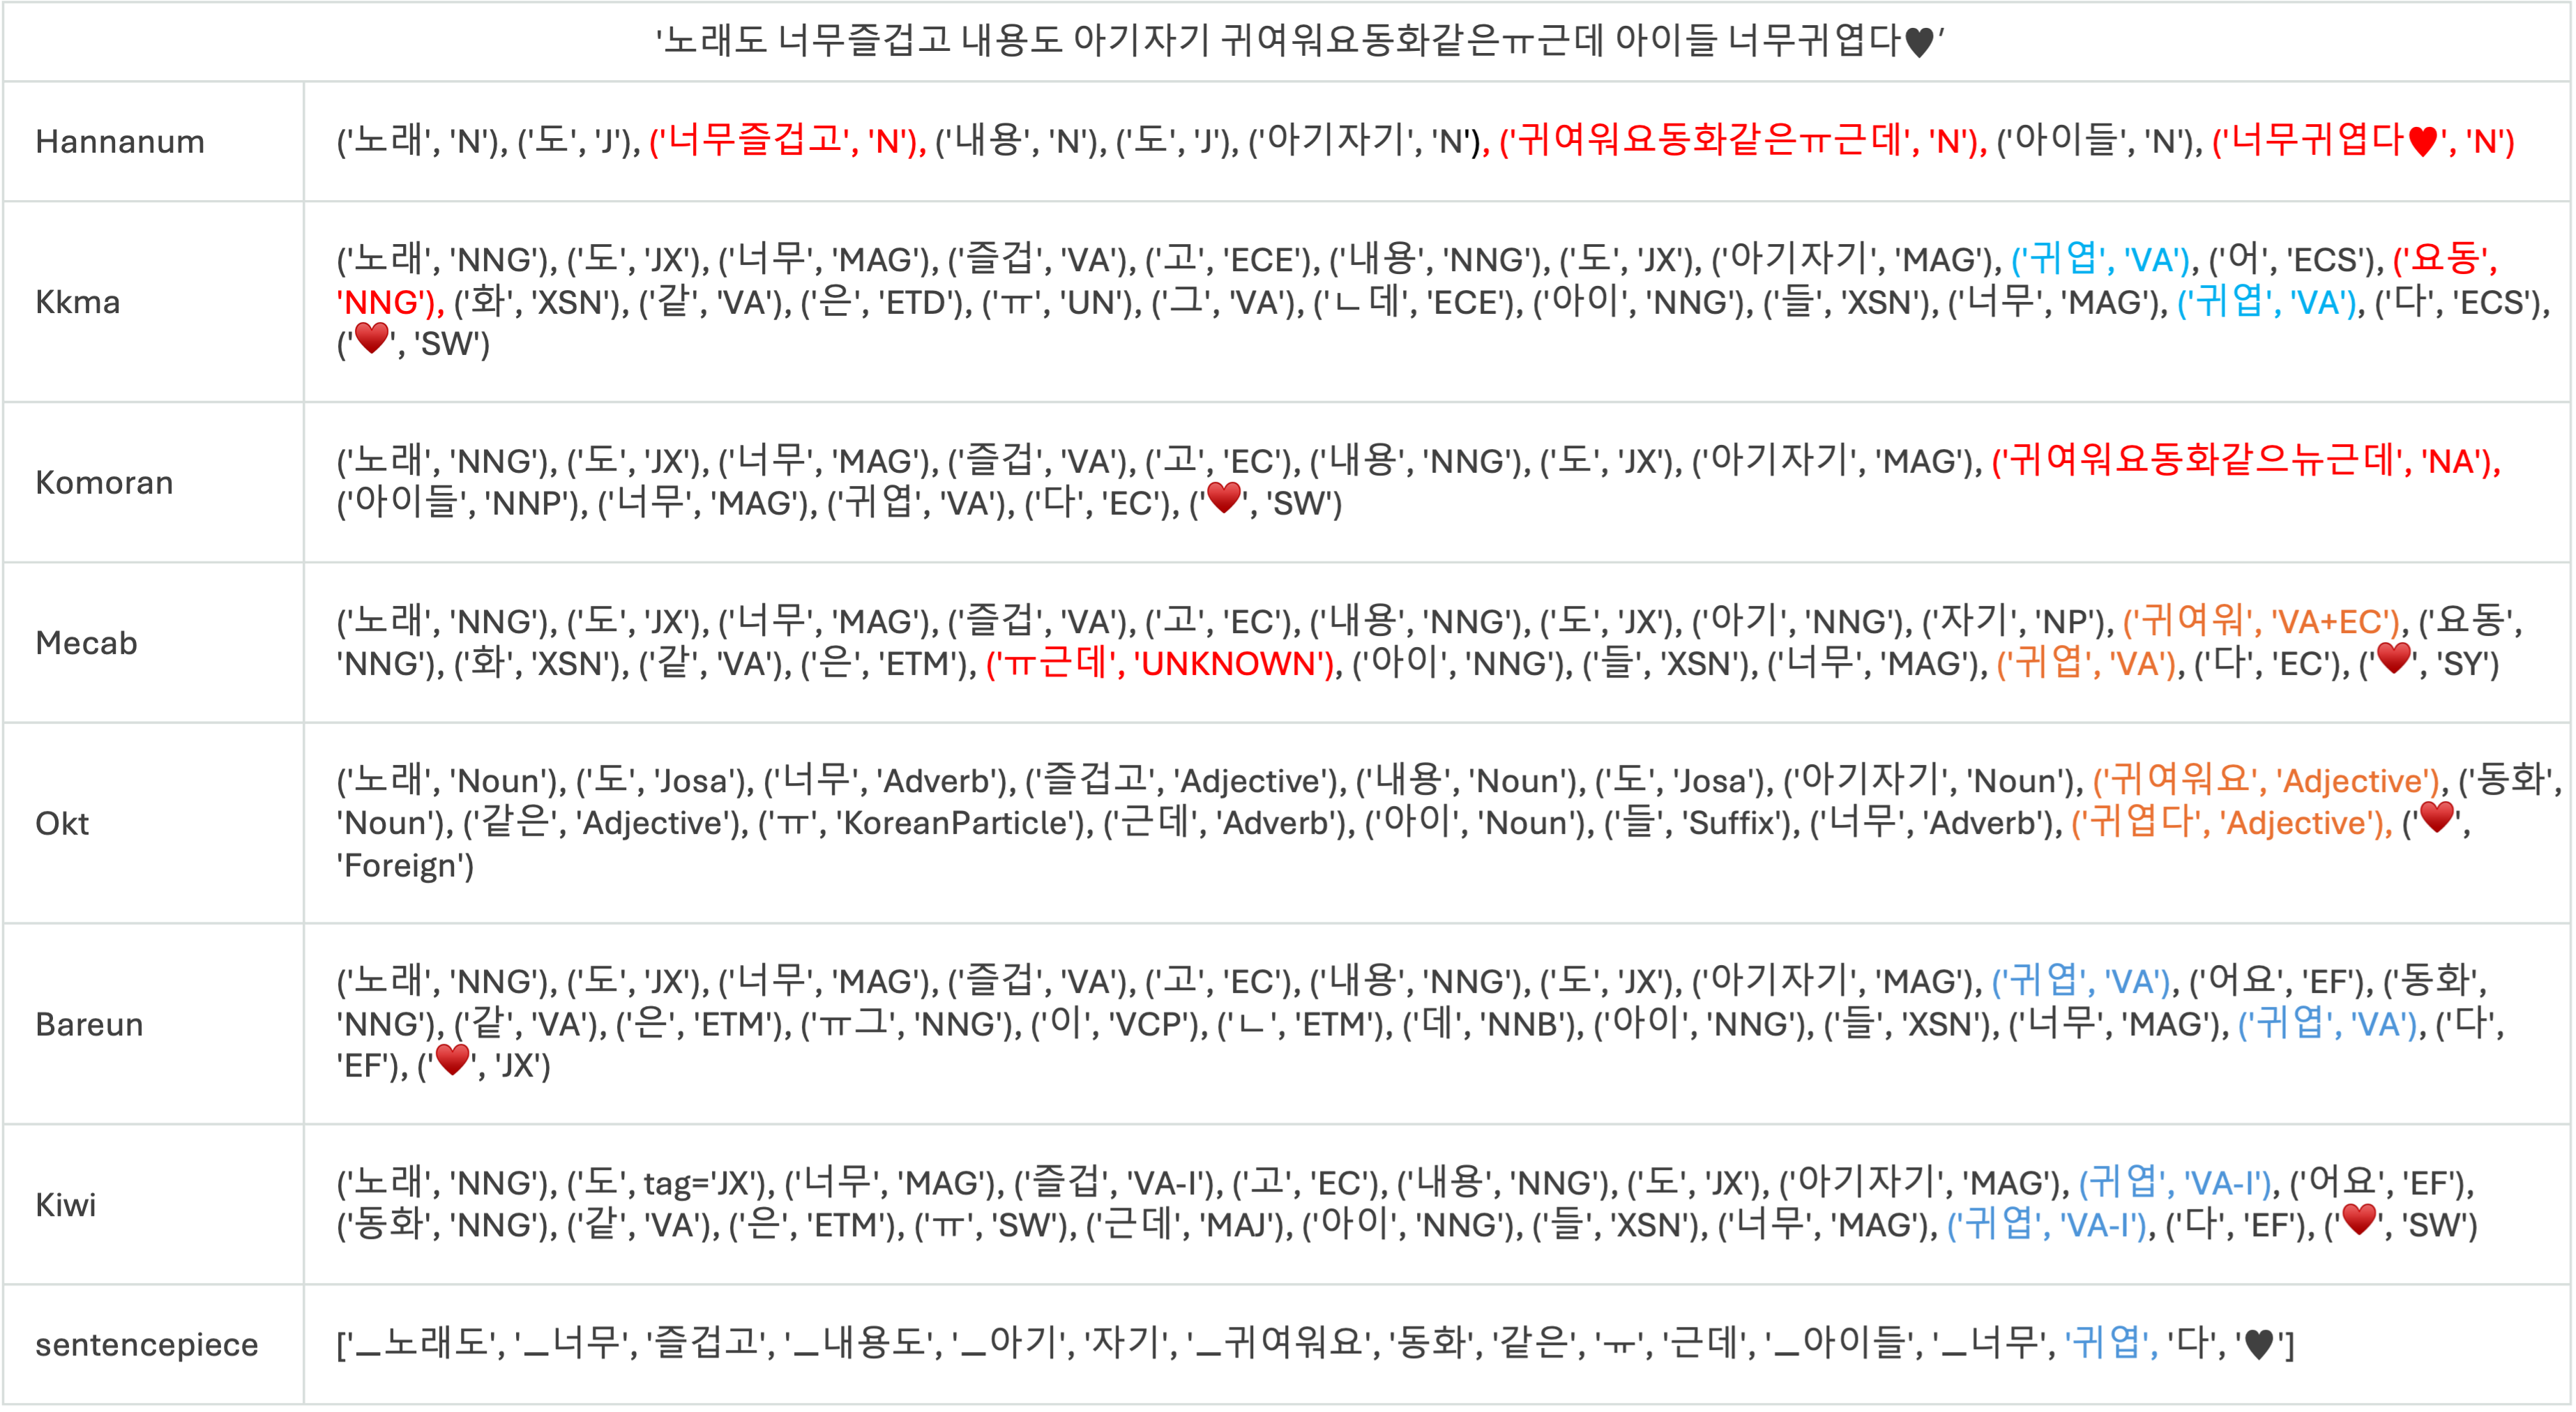
\includegraphics[width=1\linewidth]{table.png}
        \caption{Qualitative Analysis}
        \label{fig:enter-label}
\end{figure}
% \begin{table}[h!]
% \centering
% \renewcommand{\arraystretch}{1.5} % 행 간격 조정
% \begin{adjustbox}{max width=\textwidth, height=100}
% \begin{tabular}{|c|c|}
% \hline
% \textbf{Tokenizer} & \textbf{Tokenization Result} \\
% \hline
% \textbf{Hannanum} & ('노래', 'N'), ('도', 'J'), ('너무즐겁고', 'N'), ('내용', 'N'), ('도', 'J'), ('아기자기', 'N'), ('귀여워요동화같은', 'N'), ('아이들', 'N'), ('너무귀엽다❤️', 'N') \\
% \hline
% \textbf{Kkma} & ('노래', 'NNG'), ('도', 'JX'), ('너무', 'MAG'), ('즐겁', 'VA'), ('고', 'ECE'), ('내용', 'NNG'), ('도', 'JX'), ('아기자기', 'MAG'), ('귀엽', 'VA'), ('어', 'ECS'), ('동화', 'NNG'), ('같', 'VA'), ('은', 'ETD'), ('아이', 'NNG'), ('들', 'XSN'), ('너무', 'MAG'), ('귀엽', 'VA'), ('다', 'ECE'), ('❤️', 'SW') \\
% \hline
% \textbf{Komoran} & ('노래', 'NNG'), ('도', 'JX'), ('너무', 'MAG'), ('즐겁', 'VA'), ('고', 'EC'), ('내용', 'NNG'), ('도', 'JX'), ('아기자기', 'MAG'), ('귀여워요동화같은누군데', 'NA'), ('❤️', 'SW') \\
% \hline
% \textbf{Mecab} & ('노래', 'NNG'), ('도', 'JX'), ('너무', 'MAG'), ('즐겁', 'VA'), ('고', 'EC'), ('내용', 'NNG'), ('도', 'JX'), ('아기자기', 'MAG'), ('귀엽', 'VA'), ('어', 'EC'), ('동화', 'NNG'), ('같', 'VA'), ('은', 'ETM'), ('트', 'UNKNOWN'), ('너', 'NNG'), ('들', 'XSN'), ('너무', 'MAG'), ('귀엽', 'VA'), ('다', 'EC'), ('❤️', 'SY') \\
% \hline
% \textbf{Okt} & ('노래', 'Noun'), ('도', 'Josa'), ('너무', 'Adverb'), ('즐겁고', 'Adjective'), ('내용', 'Noun'), ('도', 'Josa'), ('아기자기', 'Noun'), ('같은', 'Adjective'), ('ㅠㅠ', 'KoreanParticle'), ('근데', 'Adverb'), ('아이', 'Noun'), ('들', 'Suffix'), ('너무', 'Adverb'), ('귀엽다', 'Adjective'), ('❤️', 'Foreign') \\
% \hline
% \textbf{Bareun} & ('노래', 'NNG'), ('도', 'JX'), ('너무', 'MAG'), ('즐겁', 'VA'), ('고', 'EC'), ('내용', 'NNG'), ('도', 'JX'), ('아기자기', 'MAG'), ('귀엽', 'VA'), ('어', 'EF'), ('동화', 'NNG'), ('같', 'VA'), ('은', 'ETM'), ('트', 'NNG'), ('너', 'VCP'), ('들', 'XSN'), ('너무', 'MAG'), ('귀엽', 'VA'), ('다', 'EF'), ('❤️', 'JX') \\
% \hline
% \textbf{Kiwi} & ('노래', 'NNG'), ('도', 'JX'), ('너무', 'MAG'), ('즐겁', 'VA-I'), ('고', 'EC'), ('내용', 'NNG'), ('도', 'JX'), ('아기자기', 'MAG'), ('귀엽', 'VA-I'), ('어', 'EF'), ('동화', 'NNG'), ('같', 'VA'), ('은', 'ETM'), ('트', 'SW'), ('너', 'NNG'), ('들', 'XSN'), ('너무', 'MAG'), ('귀엽', 'VA-I'), ('다', 'EF'), ('❤️', 'SW') \\
% \hline
% \textbf{SentencePiece} & ['노래도', '너무', '즐겁고', '내용도', '아기자기', '귀여워요', '동화', '같은', 'ㅠ', '근데', '아이들', '너무', '귀엽', '다', '❤️'] \\
% \hline
% \end{tabular}
% \end{adjustbox}
% \caption{Comparison of Tokenization Results from Various Tokenizers}
% \label{tab:tokenizers}
% \end{table}
       
[Figure 1] displays the tokenization results for a sample sentence using various tokenizers. Here are the summarized characteristics and performance insights for each tokenizer:

\begin{itemize}
    \item \textbf{Hannanum}: Tends to categorize many words under the single noun (N) tag, which might oversimplify the text structure.
    \item \textbf{Kkma}: Offers a wide range of part-of-speech tags, providing detailed and nuanced tokenization.
    \item \textbf{Komoran}: Generally accurate but sometimes assigns long strings to the NA tag, indicating difficulty with certain tokens, especially those lacking proper spacing.
    \item \textbf{Mecab}: Efficiently handles compound words and provides precise part-of-speech tags, showing robustness in its output.
    \item \textbf{Okt}: Uses simple and intuitive tags, making it easy to interpret, though it might lack depth in analysis.
    \item \textbf{Bareun}: Clearly distinguishes compound words and provides accurate segmentation, ensuring clarity in tokenization.
    \item \textbf{Kiwi}: Supplies detailed information about the start position and length of morphemes, allowing for fine-grained analysis.
    \item \textbf{SentencePiece}: Breaks down text into subword units, which might help with out-of-vocabulary words but can sometimes lead to less interpretable tokens.
\end{itemize}


\section{Conclusion and Future Research Directions}

\subsection{Conclusion}

This study compared Google SentencePiece and various Korean morphological analyzers. The results showed that Mecab and Soynlp were superior in speed, while Mecab, Kiwi, and Bareun exhibited high accuracy. These findings highlight the utility of morphological analyzers in Korean text processing.

\subsection{Limitations}
Since this study used a limited dataset (Naver movie review data) and did not compare using various evaluation metrics, there are limitations because it could not be compared in various aspects.

In terms of the task, there is also a question whether it is possible to measure the performance properly since it is a binary classification problem.

Also, the qualitative evaluation of tokenization quality may contain subjective factors. In addition, we were only able to experiment with a simple LSTM model, which is disappointing.

\subsection{Future Research Directions}

Future research should evaluate tokenizer performance using more diverse Korean datasets. Additionally, exploring the potential of combining morphological analyzers with subword-based tokenizers could be beneficial.

A more meaningful comparison would be to compare the effectiveness of morphological analysis on a larger model, such as the BERT (Bidirectional Encoder Representations from Transformers) language model developed by the Exobrain project, which is being promoted by the Ministry of Science and ICT and IITP's Innovation Growth Engine project, reflecting the characteristics of Korean.

We hope this paper aids in selecting the most suitable tool for Korean text processing by comparing the performance of various tokenizers.



\section{References}

\begin{itemize}
    \item \href{https://github.com/google/sentencepiece}{Google SentencePiece}
    \item \href{https://konlpy.org/}{KoNLPy Library}
    \item \href{https://bareun.ai/}{바른}
    \item \href{https://github.com/lovit/soynlp}{Soynlp}
    \item \href{https://github.com/bab2min/Kiwi}{Kiwi}
    \item \href{https://aiopen.etri.re.kr/bertModel}{Bert Korean Model}
\end{itemize}

\section{Appendix}

\subsection{Additional Sentence Piece results}

\begin{itemize}
\item vocab size = 8000, model type variation
    \begin{itemize}
        \item lstm model : 0.8601
        \item stacked lstm model : 0.8517
        \item 1d cnn model : 0.8557
    \end{itemize}

\item SentencePiece vocab size, type variation (lstm model)
    \begin{itemize}
        \item increase vocab size to 21741 : 0.8608
        \item change model type to bpe : 0.8601
    \end{itemize}
No significant change in performance improvement

\end{itemize}

\subsection{Roc Curve of Test [Figure 2]}
To compare the performance of the new tokenizers, kiwi, bareun, soynlp's ltokenizer, and max score tokenizer, we additionally ran a roc curve to check their performance
\begin{figure}
    \centering
    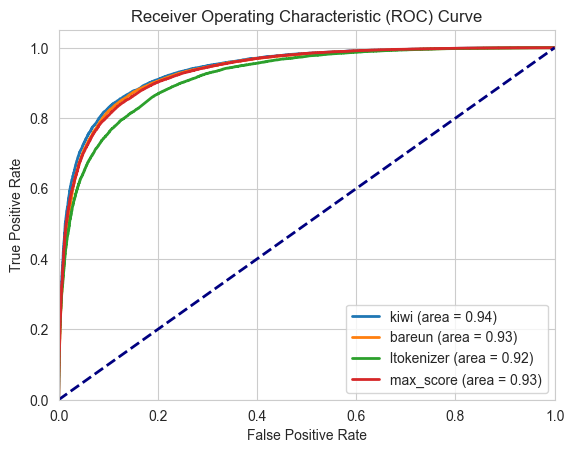
\includegraphics[width=0.6\linewidth]{roc_curve.png}
    \caption{Roc Curve}
    \label{fig:enter-label}
\end{figure}

\subsection{Execution Time Comparison [Figure 3]}
The graph below([Figure 3]) is a text analysis speed comparison graph provided by \href{https://github.com/bab2min/Kiwi?tab=readme-ov-file}{Kiwi}. You can see that this graph shows similar results to what we found in our previous study

\begin{figure}
    \centering
    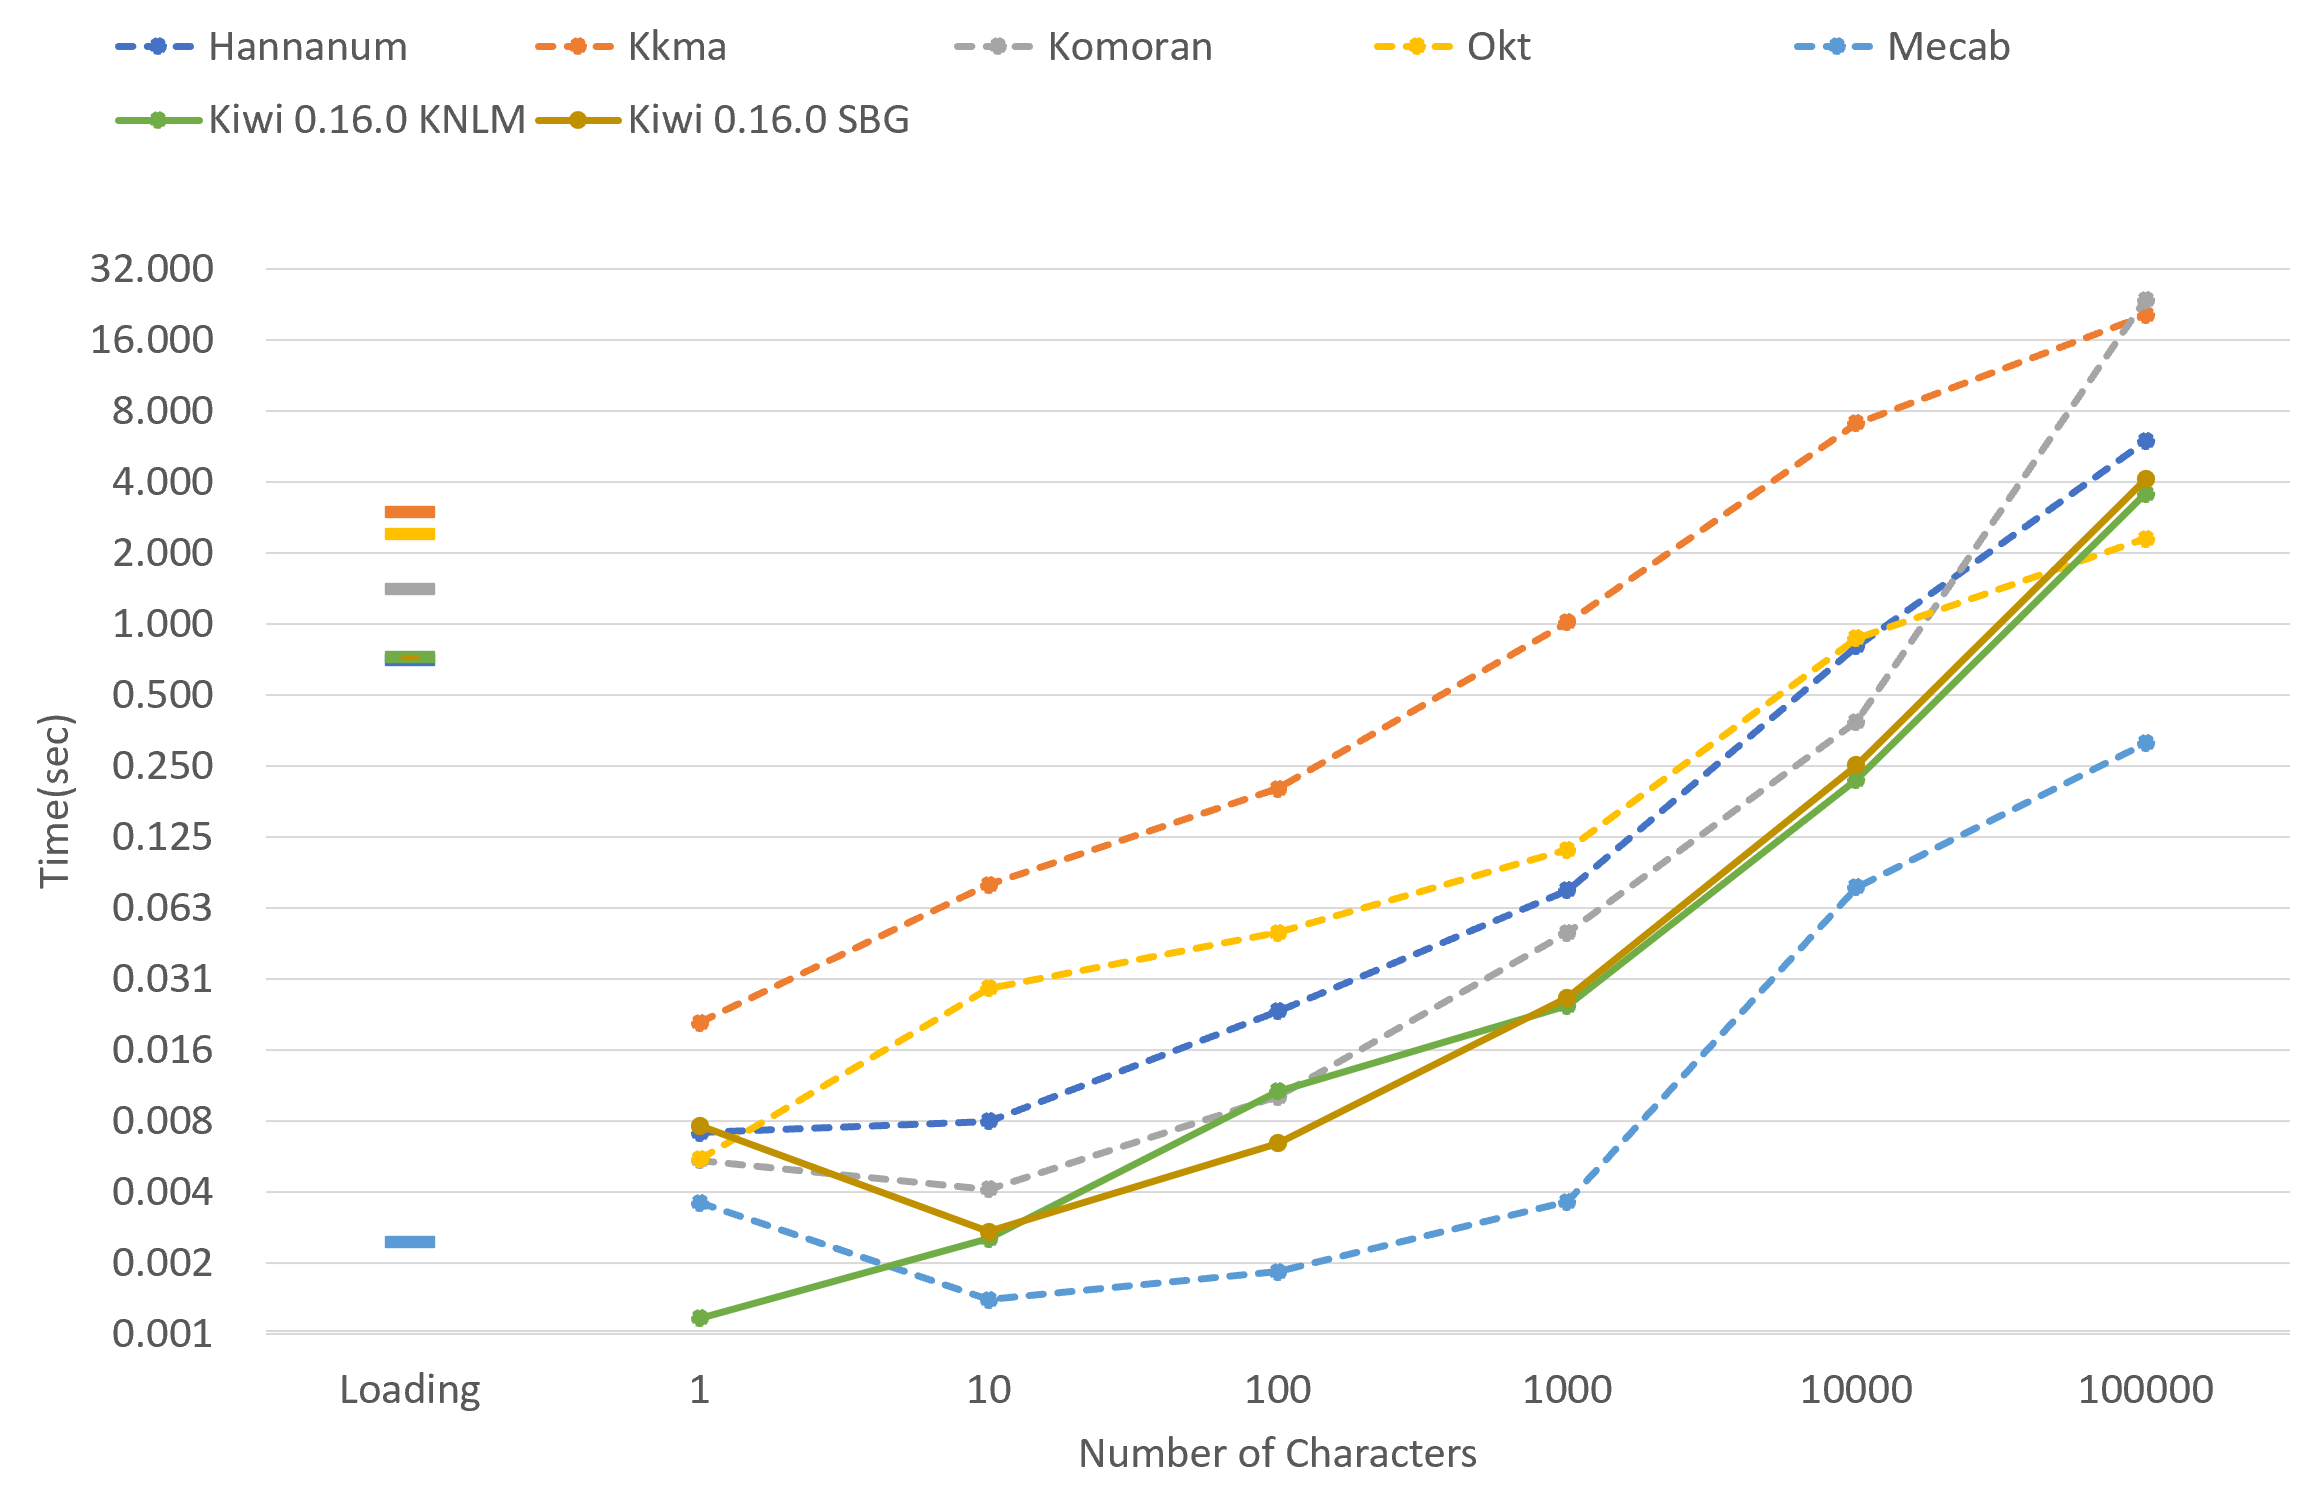
\includegraphics[width=0.6\linewidth]{compare_speed.png}
    \caption{Execution Time Comparison}
    \label{fig:enter-label}
\end{figure}

\end{document}
